%!TEX root = ../master.tex
\section{Functional programaing}

\subsection{(Untyped) Lambda Calculus}
\label{Lambda Calculus}
Lambda calculus is a collection of formal systems for expression computation and is a basis for functional programming. Alonzo Church introduced lambda calculus in the 1930s and published his first book on the topic in 1941 \autocite{ChurchAlonzo1985Tcol}. Furthermore, lambda calculus is a universal model of computation that can express any computable function, resulting in it being Turing complete. We base the following section on \autocite{RojasRaulLC} and \autocite{nederpelt_geuvers_lc}. 

\subsubsection{Definitions and notations}
Lambda calculus consists of three primitives symbols: $\lambda$, (, and ). The fundamental concept in lambda calculus is a lambda term, also called an expression. A lambda term may consist of: 

\begin{itemize}
    \item \textbf{Variable}: A name which  is a placeholder for a parameter. A variable $x$ is in itself a lambda term.
    \item \textbf{Abstraction}: If we have a term $M$ and an variable $x$, then we also have the term $\lambda x.M$ where $x$ is bound in M. 
    \item \textbf{Application}: If $E_1$ and $E_2$ are lambda terms, then $(E_1 E_2) $ is also a lambda term, where $E_2$ is applied to $E_1$.
\end{itemize}

Lambda calculs buildes up its $lambda$-terms using these three expressions, which in BNF-syntax can be defined as: 

\begin{table}[ht!]
    \centering
    \begin{tabular}{c c c}
         $\lambda -term$ & $:= $& <variabel> \\
         & $|$ & <abstraction> \\
         & $|$ & <application> \\
    \end{tabular}
\end{table}

\para
All functions in $\lambda$-calculus are first-class values, which means that a lambda function can take in a function as an argumnent and returning functions. Bear in mind that $\lambda$-calculus is left-associative, which means that $E_1 E_2 E_3 \leftrightarrow E_1 (E_2 E_3)$.

\para
In the following sections, refer to \autoref{fig:LC-explenations} for simple visualization of the different parts of a lambda function. 
\begin{figure}
    \centering
    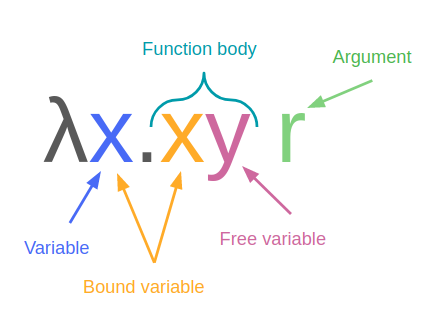
\includegraphics[scale=0.4]{lambdaCalculusFunctionExplenation.png}
    \caption{Visualization of the different parts of a lambda function}
    \label{fig:LC-explenations}
\end{figure}

\subsubsection{Bound and Free variables}
As previously mentioned, the \emph{abstraction} sets the \emph{bound variables}. Within the abstraction, if the variable exists in the function body, the $\lambda$ binds this variable to the function body. For example, given the term $\lambda x.xy$, $x$ is a bound variable because: $x$ occurs in the function body, and $\lambda$ binds $x$ to the function body.

\para
\emph{Free variables} are the opposite of bound variables. Formally, we can say that if we have a term $E_1$ with a set $V_1$ for all variables and $B_1$ for bound variables; 
then the free variables $F_1$ are $F_1 = V_1\setminus B_1$. We can also extend this general rule further, 
by adding another term $E_1$ with a set $V_2$ for all variables and $B_2 $ for all the bound variables;
then the \emph{free variables} in $E_1 E_2$, $F_1 F_2$ equals $ (V_1\setminus B_1) \cup (V_2\setminus B_2)$. 
In other words, the set of free variables in the term $E_1 E_2$ is the union of the free variables in $E_1$ and $E_2$.

\subsubsection{$\alpha$-conversion}
To explain $\alpha$-conversion, one needs to understand what \emph{$\alpha$ equivalence} is. In short, two lambda terms are $\alpha$-equivalent if the only difference in the terms has the variables' names. E.g $\lambda ab.ab$ is alpha-equivalent to the lambda term $\lambda xy.xy$ 

\para
With $\alpha$-equivalent in mind, \emph{$\alpha$-conversion} is a way to change a variable name in both the $\lambda$ part and the function body while keeping the new term $alpha$ equivalent to the old term. E.g. $\alpha$-conversion of $\lambda ab.ab$ is $\lambda xy.xy$ since these are $alpha$ equivalent. Bear in mind that changing a variable name to an already existing variable name in the term is not allowed, because the result would change the meaning and thus the two terms would not be $alpha$ equivalent.

\para
As we have already mentioned, when doing $\alpha$-conversion, we can only change the names of the variables in the term so that the term does not change its meaning. 
E.g., $\lambda x.x \rightarrow_\alpha \lambda y.y$ since we have not changed the meaning of this term. The result of sending in any value/term $e$ will give us the same return value, in this case, just $e$ itself. An example of what is not allowed to do is this $\lambda x.xy \rightarrow_\alpha \lambda y.yy$, as these terms will give us different return values for an argument. Let us try with $e$ again; then we would see that  $\lambda x.xy e$ would give us $ey$ while $\lambda y.yy e$ would give us $ee$, and $ey \neq ee$. So the term $\lambda x.xy$ is $\alpha$-equivalent to all terms where we change to $x$ to anything except $y$. We can generally change any variable name to anything except the set of variables in the function body. Therefore $\lambda x.xy \rightarrow_\alpha \lambda z.zy$. Besides, we need to make sure that we only changes the variables that are in the same abstraction. So the term $\lambda x.\lambda x.x $ is not $\alpha$-equivalent to the 
term $\lambda y.\lambda x.y$, but to for example the terms $\lambda y.\lambda x.x$ or $\lambda x.\lambda y.y$.

\subsubsection{$\beta$-reduction}
$\beta$-reduction is a way to reduce terms. We reduce terms by sending in argument(s) for the bound variables. E.g., if we want to reduce the lambda term $\lambda x. x s$, 
we can $\lambda x. x$  $s \rightarrow _\beta s$ (this is the identity function, which gives us back the argument we gave to the function). We can do $\beta$-reduction in several rounds. When there are no more possible $\beta$-reductions, we say that the term has reached the $\beta$-normal form. \autoref{fig:beta-reduction} shows an example on $\beta$-reduction with a $\lambda$-term of one of the arguments. 

\para
Futhermore, we say that a term, M, is \emph{$\beta$-equal} to another term, N, if finite $\beta$-reductions on the term M results in the term N. This is often denoted with $M =_{\beta} N$. In \autoref{fig:beta-reduction} the term $\lambda x.\lambda y. xy \; (\lambda z.z) \; a \; b$ is $\beta$-equal to all the terms beneath. 

\para
If the term stays the same after one $\beta$-reduction, the term will never terminate. An example of a term that does not terminate while using $\beta$-reduction is the self-application function applied on itself $(\lambda f.ff) \lambda f.ff$.

\paragraph{Complexity}
$\beta$-reduction is not an atomic step; this means that one must locate all occurrences of a bound variable in a term, which can be very time-consuming. In O-notation, this will take $O(n)$ time for a term of length n. Also, storing all of these occurrences may become costly in regards to storage. 

\begin{figure}
    \centering
    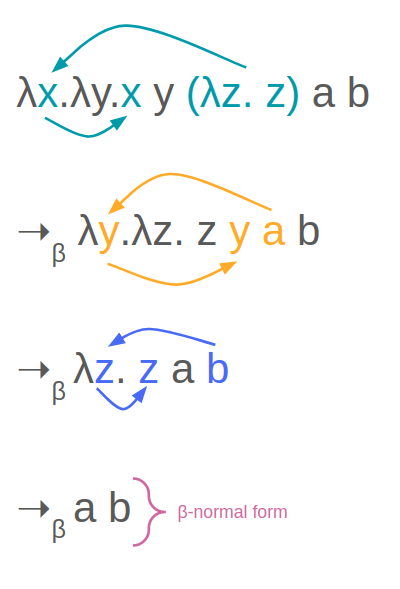
\includegraphics[scale=0.4]{b-reduction.png}
    \caption{An example of $\beta$-reduction}
    \label{fig:beta-reduction}
\end{figure}

\subsubsection{$\eta$-reduction}
$\eta$-reduction is the idea that two functions are equal if, and only if, they return the same result for any given argument. An example of $\eta$-reduction is $(\lambda x.f x)  \rightarrow_\eta f$, whenever $x$ is not a free variable in $f$.

\subsection{Combinatory logic}
\label{combinatory logic}
Combinatory logic in computer science, is a theoretical method of computation. The idea is that we only have some base function to create new high-order functions. From now on, these functions will be called primitive functions. These primitive functions combined in the proper order can then express any other high-order function. Combinatory logic is often looked at as a variant of $\lambda$-calculus, where the lambda expressions are replaced with a limited set of primitive functions that does not have any free variables. 
The three primitive functions in combinatory logic is \textbf{I}, \textbf{K} and \textbf{S}.
\\ \\
Where \textbf{I} is the identity function, defined by: \\ 
\begin{center}
    $(I x) = x$\\    
\end{center}
Written in $\lambda$-calculus, the \textbf{I} function would look like this:\\
\begin{center}
    $\lambda x.x$\\    
\end{center}
Futhermore, we have the \textbf{K} function that takes in two arguments and always returns the first argument, defined by:
\begin{center}
    $ ((K x) y) = x$ or $(K x y) = x$\\    
\end{center}
Written in $\lambda$-calculus, the \textbf{K} function would look like this:\\
\begin{center}
    $\lambda xy.x$\\    
\end{center}
Lastly, we have the primitive function \textbf{S}, which takes in three arguments and applies the last argument on the two first arguments:
\begin{center}
    $ (S x y z) = (x z (y z))$\\    
\end{center}
Written in $\lambda$-calculus, the \textbf{S} function would look like this:\\
\begin{center}
    $\lambda xyz.xz(yz)$\\    
\end{center}
From these primitive functions and a variable $x$, we can build up combinatoric terms as shown in \autoref{tab:makeCombinatoricTerms} almost the same way that we build up different terms in $\lambda$-calculs. The difference between combinatoric logic and $\lambda$-calculus, is that we have a limited set of primitive functions in combinatoric logic, and in $\lambda$-calculus we have abstractions.

\begin{table}[]
    \centering
    \begin{tabular}{c c c | c}
         $E :=$&  & $x$ & (variable)\\
         & $|$ & $P$ & (the primitive functions) \\
         & $|$ & $E_1 E_1$ & (application, where $E_1$ and $E_2$ are combinatoric terms)\\
    \end{tabular}
    \caption{How to build up combinatoric terms}
    \label{tab:makeCombinatoricTerms}
\end{table}

\para
If we want to convert a lambda term to an equivalent combinator, we use a transformation $T[]$, which is defined by the following rules:
\begin{enumerate}
    \item $T[x] \Rightarrow x$
    \item $T[(E_1 E_2)] \Rightarrow (T[E_1]\; T[E_2])$
    \item $T[\lambda x.E] \Rightarrow (\textbf{K}\; T[E])$ (if x dosen't occure free in E)
    \item $T[\lambda x.x]\Rightarrow \textbf{I}$
    \item $T[\lambda x. \lambda y.E]\Rightarrow T[\lambda x.T[\lambda y.E]]$ (if x occures free in E)
    \item $T[\lambda x.(E_1 E_2)] \Rightarrow (\textbf{S} \; T[\lambda x.E_1] \; T[\lambda x.E_2])$
\end{enumerate}
T[] is not a well-typed mathematical function but a rewriter, which means that an uncompleted transformation will result in something that is neither a lambda term nor a combinatory term. 

\para
The following example explains how to transform the expression $\lambda x.\lambda y.xy$ from \autoref{fig:beta-reduction}. Note that we have made one shortcut to save time. The shortcut combines rule 3 and 1, which we write as $3/1$ in the example below.
In consequence, $T[\lambda x.y]$ we write $T[\lambda x.y] =_{3/1} (\textbf{K } y)$ instead of $T[\lambda x.y] =_{3} (\textbf{K } T[y]) =_{1} (\textbf{K } y)$.
\begin{quote}
    $\lambda x.\lambda y.xy$ \\
    $=_5 T[\lambda x.T[\lambda y.(xy)]]$ \\
    $=_6 T[\lambda x. (\textbf{S}\; T[\lambda y.x]\; T.[\lambda y.y])]$ \\
    $=_{3/1} T[\lambda x. (\textbf{S}\;(\textbf{K}\; x) \; T.[\lambda y.y])]$ \\  
    $=_4 T[\lambda x. (\textbf{S}\;(\textbf{K}\; x) \; \textbf{I})]$ \\
    $=_6 (\textbf{S} \; T.[\lambda x.(\textbf{S}\;(\textbf{K}\; x))] \; T.[\lambda x.I])$ \\
    $=_{3/1} (\textbf{S} \; T.[\lambda x.(\textbf{S}\;(\textbf{K}\; x))] \; (\textbf{K I}))$ \\
    $=_{6} (\textbf{S} \; (\textbf{S} \; T[\lambda x.\textbf{S}] \; T[\lambda x.(\textbf{K} \; x)]) \; (\textbf{K I}))$ \\
    $=_{3/1} (\textbf{S} \; (\textbf{S} \; (\textbf{K S}) \; T[\lambda x.(\textbf{K} \; x)]) \; (\textbf{K I}))$ \\
    $=_{6} (\textbf{S} \; (\textbf{S} \; (\textbf{K S}) \; (\textbf{S} \; T.[\lambda x.\textbf{K}] \; T.[\lambda x.\textbf{x}]) ) \; (\textbf{K I}))$ \\
    $=_{3/1} (\textbf{S} \; (\textbf{S} \; (\textbf{K S}) \; (\textbf{S} \; (\textbf{K K}) \; T.[\lambda x.\textbf{x}]) ) \; (\textbf{K I}))$ \\
    $=_4 (\textbf{S} \; (\textbf{S} \; (\textbf{K S}) \; (\textbf{S} \; (\textbf{K K}) \; \textbf{I}) ) \; (\textbf{K I}))$ \\      
\end{quote}
It is common to add the combinatory terms \textbf{B} ($(\textbf{C} f g x) = ((f x )g)$) 
and \textbf{C} ($(\textbf{C} f g x) = (f (x g))$). \textbf{C} performes substitution on the the first term, and \textbf{B} on the second term, in contrast to \textbf{S} which performs substitution on both terms. These two terms can now be added to the transformation, $T[]$:
\begin{enumerate}
    \setcounter{enumi}{6}
    \item $T[\lambda x.(E_1 E_2)] \Rightarrow (\textbf{C} \; T[\lambda x.E_1] \; T[E_2]))$ (if x is free in $E_1$ but not in $E_2$)
    \item $T[\lambda x.(E_1 E_2)] \Rightarrow (\textbf{B} \; T[E_1] \; T[\lambda x.E_2])$ (if x is free in $E_2$ but not in $E_1$)
\end{enumerate}
\textbf{B} and \textbf{C} are define as the following using the primitive functions:\\
$\textbf{B=(S(K S)K)}$\\
$\textbf{C=(S(S(K(S(K S)K))S)(K K))}$\\

\subsection{Type theory}
\label{type theory}
Type theory is the academic study of \emph{type systems}, which gives every term a type. The type determines the meaning, and which operations are possible to perform on a term. Lambda Calculus has its own type system, also made by Alonzo Church called \emph{Simply Typed Lambda Calculus}, which we discuss in \autoref{Simply Typed Lambda Calculus}.

\para
\emph{A term} is often followed by a : and then the type of the term. \emph{A type} in a type system is semantically a collection of different values that a term can be evaluated to be. Therefore, there are many similarities between type systems and set theory, although they have their differences. Furthermore, the name of a given term is syntactic. For example, in java, where we have a type that is a collection of all Integers ($\mathbb{Z}$) (semantic) and has the name int (syntactic). Consequently, a term $e$ ($e$ is often used to denote a term) is of type $\tau$ ($\tau$ is often used to denote a type) if $e \in \tau$. E.g. 2 is of type $\mathbb{N}$ (natural numbers) because $2 \in \mathbb{N}$. Making new types depends on the type systems' set of base types and type constructors, often called the \emph{inductive types} of a type system. An example type system with the base type $\sigma$, two type constructors $*$ and $\#$, and two types $M$ and $N$, makes it possible to make a new type $T$ as shown in \autoref{tab:inductive types}. 

\para
Many of the programming languages using type systems either require that all expressions terminate (e.g. Coq) or allow infinite loops but are inconsistent when viewed as logics (e.g. Haskel) \textbf{(src: http://www.tyconmismatch.com/papers/combining-TR.pdf)}.
Therefore in some programming languages like \nameref{Simply Typed Lambda Calculus}, one of the type systems goals is to make sure that a term terminates. 

\begin{table}[]
    \centering
    \begin{tabular}{c c c}
         $T :=$&  & $\sigma$\\
         & $|$ & $M * N$ \\
         & $|$ & $M \# N$ \\
    \end{tabular}
    \caption{Example of how to build up inductive types}
    \label{tab:inductive types}
\end{table}


\subsubsection{Decision problems}
Type theory uses type checking, typability and type inhabitation as decisions problems. These decision problems uses judgments, which are denoted with $\Upgamma \vdash e:\tau$. Where $\Upgamma$ is the denotation which is usually used for a context or environment. A terms' type is determined using the judgment and equivalences type inference rules. 

\para
The decision problem of \textbf{checking} (abbreviated by ($\Upgamma\vdash e : \tau$?) is:\\
\textit{Given a type environment $\Upgamma$, a term $e$, and a type $\tau$, decide whether the term $e$ can be assigned the type $\tau$ in the type environment $\Upgamma$} \\ \\
The decision problem of type \textbf{typability} (abbreviated by ($ \exists \Upgamma,\tau .\Upgamma\vdash e : \tau$?) is: \\ 
\textit{Given  a term $e$, decide wheter there exists a type environment $\Upgamma$ and a type $\tau$ such that the term $e$ can be assigned the type $\tau$ in the type environment $\Upgamma$} \\ \\ 
The decision problem of type \textbf{inhabitation} (abbreviated by ($ \exists e.\Upgamma \vdash e : \tau$?) is: \\
\textit{Given a type environment $\Upgamma$ and a type $\tau$, decide whether there exists a term $e$ that can be assigned the type $\tau$ in the type environment $\Upgamma$}

\subsection{Simply Typed Lambda Calculus}
\label{Simply Typed Lambda Calculus}
As we mention in \autoref{type theory}, Simply Typed Lambda Calculus($\lambda^\rightarrow$) is a Type Theory developed by Alonzo Church for lambda-calculus. In $\lambda^\rightarrow$, we can make types with only one constructor $\rightarrow$ and a set of base types, frequently denoted with a $B$. Thus, we can construct new types from the base types, $B$, combined with constructor $\rightarrow$. Using base types $\tau$ and $\sigma$, for instance, make it possible to construct type $\tau \rightarrow \sigma$. $\tau \rightarrow \sigma$ refers to a function that takes in a term of type $\tau$ and returns a term of type $\sigma$, such as: $\lambda x:\tau. y \; \tau \rightarrow \sigma$. 


\para
The syntax for Simply Typed Lambda Calculus is almost identical to Lambda Calculus, with the difference being that we need to define the variables' type in the abstraction. Simply Typed Lambda Calculus similarly specifies the variables' type as in type theory, with $x:\tau$ for a variable $x$ with type $\tau$. In addition, Simply typed lambda calculus adds a set of term constants for the base types, often denoted with a $c$. \autoref{tab:STLC syntax} shows the complete syntax for Simply Typed Lambda Calculus.


\begin{table}[]
    \centering
    \begin{tabular}{c c c}
         $e :=$&  & $x$\\
         & $|$ & $\lambda x:\tau.M$ \\
         & $|$ &  $M N$ \\
         & $|$ &  $c$ \\
    \end{tabular}
    \caption{Simply Typed Lambda Calculus syntax}
    \label{tab:STLC syntax}
\end{table}

\subsubsection{Typing rules}
Simply Typed Lambda Calculus has four typing rules. To state these rules, Simply Typed Lambda Calculus uses the typing environment we define in \autoref{type theory}. The four typing rules are:

\begin{enumerate}
    \item If we have variable $x$ that is of type $\tau$ in the typing environment $\Upgamma$, then we know that $x$ has type $\tau$.
    \item If we have a constant $c$ of type $T$ in the typing environment $\Upgamma$, then we know that $c$ has type $T$.
    \item If we have a variable $x$ of type $\tau$ in a type environment $\Upgamma$, and a term $e$ of type $\sigma$ in $\Upgamma$; then we have a term $\lambda x\tau .e$ with the type $\tau \rightarrow \sigma$ in $\Upgamma$.
    \item If we have a term $M$ of type $\tau \rightarrow \sigma$ and a term $N$ of type $\tau$ in an typing environment $\Upgamma$; then $M N$ will have the type $\sigma$ in $\Upgamma$.
\end{enumerate}

\subsubsection{Reduction of Simply Typed Lambda Calculus}
Simply Typed Lambda Calculus also uses the $\beta$-reduction and $\eta$-reduction as \autoref{Lambda Calculus} mention. Additionally, the reduction needs to check that the arguments to the function have the right type in typing environment. 

\para
To give an example of $\beta$-reduction, we first need to make a set of the base types. In this case, we only use $Int$, the collection of all-natural numbers. From $Int$, it is possible to make an unlimited set of types, such as $Int$, $Int \rightarrow Int$, $Int \rightarrow Int \rightarrow Int$. For the sake of this example, we add the operation $+$ that adds two numbers together. We use the term $e_1:= \lambda x:Int\: y:Int. + x y:Int \rightarrow Int \rightarrow Int$. The type $Int \rightarrow Int \rightarrow Int$ is a term that takes in an Int and returns a term that takes in an $Int$ and returns an $Int$. Applying $e_2 := 3:Int$ with the third typing rule on the term $e_1$, $e_1 e_2$ results in the term $e_1 e_2$ with the type $Int \rightarrow Int$. This type describes a term that taks in a Int and returns a Int, which we can be prove using $\beta$-reduction on the term:
\\ \\
$e_1 e_2 := (\lambda x:Int\: y:Int. + x y:Int \rightarrow Int \rightarrow Int)\; 3:Int 
\newline\rightarrow_\beta \lambda y:Int. + 3\; y: Int \rightarrow Int$
\\ \\
Again, using the third typing rule and applying $e_3 := 7:Int$ on the term $e_1 e_2:Int \rightarrow Int$ results in the term $e_1 e_2 e_3$ with the type $Int$, proven by $\beta$ reduction: 
\\ \\
$e_1 e_2 e_3 := (\lambda y:Int. + 3\; y: Int \rightarrow Int) \; 7:Int
\newline \rightarrow_\beta + 3:int \; 7:Int = 10$

\subsection{Evaluation strategies}
\emph{Evaluation strategies} are a collection of strategies that decides when a programming language should evaluate an expression. An evaluation strategy chooses, among other things, if the language should evaluate expressions sent into a function before executing the function or send in these expressions and evaluate them at a later stage.

\para
Evaluation strategy has two main strategies \emph{eager evaluation} (strict evaluation) and \emph{non-strict evaluation}. To briefly explain, the eager evaluation evaluates the expression as soon as it is bound, while the non-strict evaluation evaluates the expression as soon as it is utilised.Meaning that eager evaluation evaluates arguments of a function, although these arguments may never be used. Non-strict evaluation can also handle infinite lists, also called streams, because non-strict evaluation only evaluates elements that are used. In this case, the eager evaluation would evaluate forever. Additionally, the eager evaluation evaluates the expression as soon it is bound. Therefore, eager evaluation only evaluates an expression once, regardless of how many times a program utilises it. Non-strict evaluation, on the other hand, ends up evaluating the exact expression n times, where n is how many times the expression is used.

\para
Most Imperative programming languages use eager evaluation because it is easy to avoid unexpected behaviour and conduct debugging compared to non-strict evaluation. It may be challenging to use imperative features like I/O and exception handling when using a non-strict evaluation strategy due to state handling. Although most imperative languages use eager evaluation, they often utilise some non-strict evaluation methods. An excellent example of this is the if-statement. In most languages, the if-statement only evaluates the part of the statement that is true. For instance, the pseudo-code, $if\; a\; then\; b\; else\; c$, will only evaluate $b$ if $a$ evaluates to be true. $c$, on the other hand, will only be evaluated if $a$ is false. However, suppose the if-statement is put into a function and use $a$, $b$, and $c$ as arguments, like $f(a, b,c):= \; if\; a\; then\; b\; else\; c$. In that case, the eager evaluation evaluates all the expressions before running the function; despite that, the programming language only needs to evaluate either $b$ or $c$. While non-strict evaluation, on the other hand, only evaluates the used expressions.

\para
\emph{Lazy evaluation}, also known as call-by-need, is a type of non-strict evaluation often used by functional programming. The result of lazy evaluation being a type of non-strict evaluation is that lazy evaluation evaluates the expression when used. What separates lazy evaluation from the other types of non-strict evaluation, such as call-by-name, is that lazy evaluation also uses memorisation to avoid repeated evaluations.  Memorisation uses a look-up table where the evaluated value of a function for some given arguments is stored.  When lazy evaluation evaluates an expression, it first checks if the expression already exists in the look-up table. If the value exists, lazy evaluation retrieves the value from the table. However, if the value is not present in the look-up table, lazy evaluation evaluates the function to a value and appends this value to the table. 

\para
\autoref{fig:strictVSLazy} is an example of strict evaluation and lazy evaluation with b-reduction. Note the following significant differences between these two approaches in this example:

\begin{itemize}
    \item Strict evaluation evaluates an expression (terms) as soon as it is bound. In contrast, lazy evaluation waits until the expression is used.
    \item Strict evaluation evaluates the expressions (terms) before sending them into the term, while lazy evaluation takes in the whole expression.
    \item On the last two lines in \autoref{fig:strictVSLazy}, lazy evaluation uses memorisation to retrieve the return value rather than evaluating it.
\end{itemize}


\begin{figure}
    \centering
    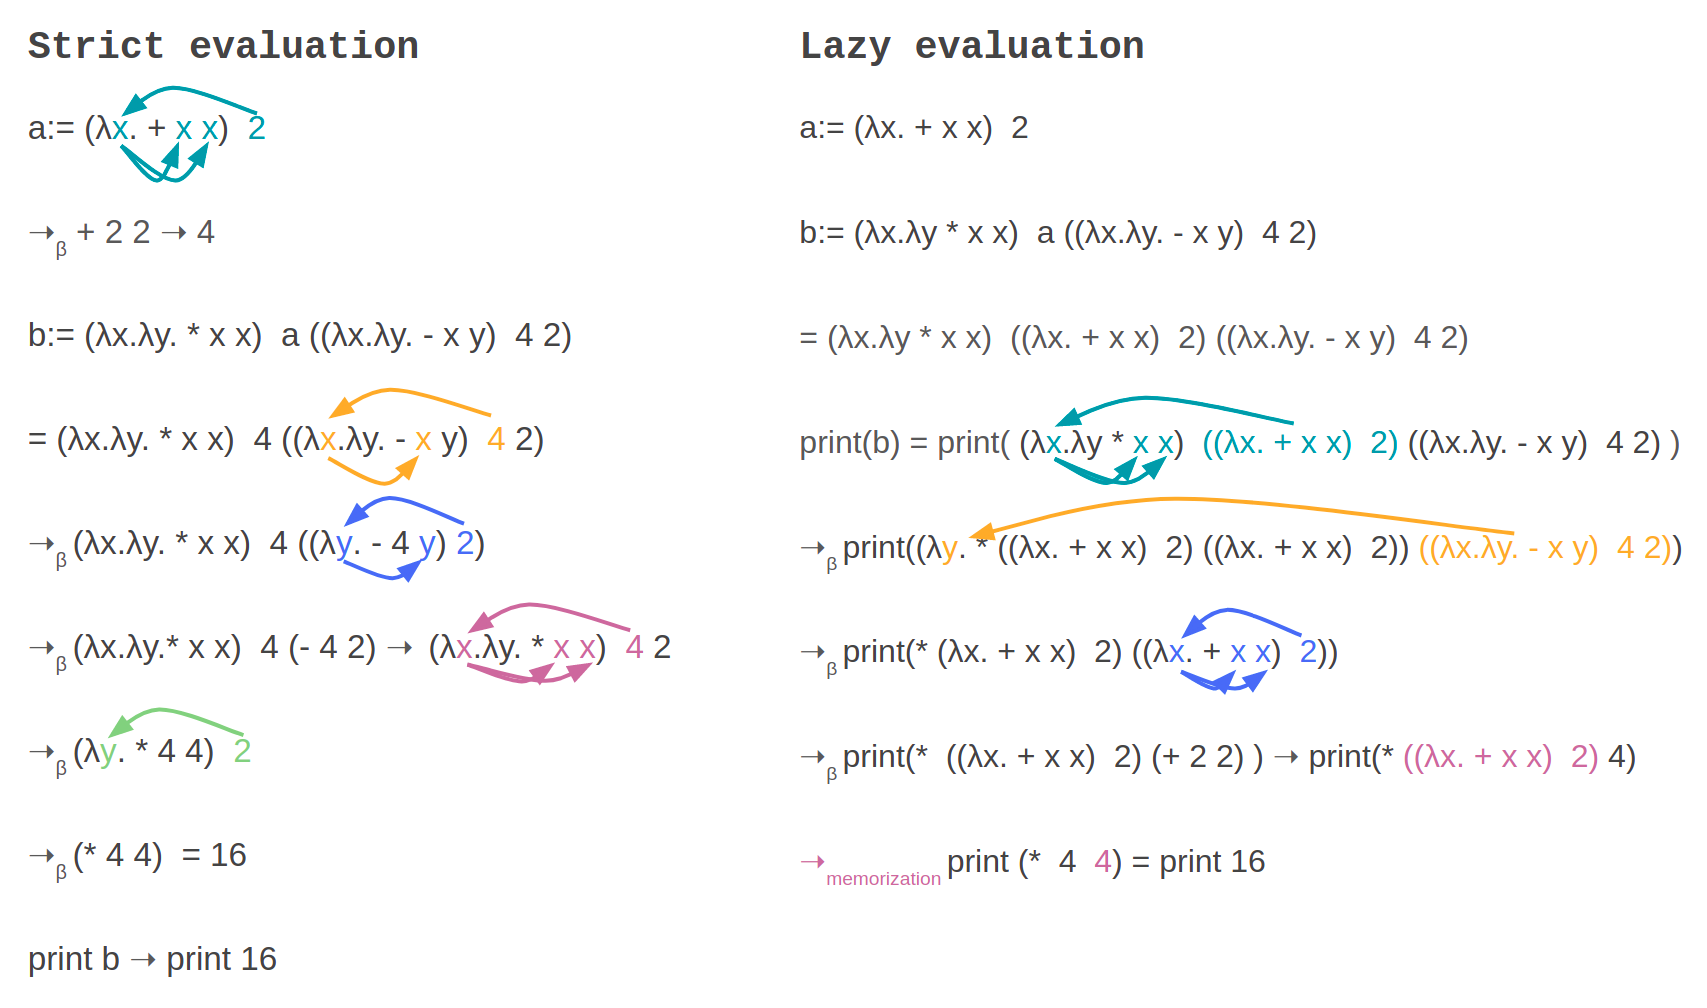
\includegraphics[scale=0.25]{strictVSLazy.png}
    \caption{Shows the difference between strict evaluation and lazy evaluation. Here we assume that print is a term which prints the argument to the terminal, and that +, -, and * are operators that work on integers}
    \label{fig:strictVSLazy}
\end{figure}

\subsection{Practical use of functional programming}
\emph{Functional programming} is a programming paradigm that is made by applying and composing functions. Furthermore, functional programming is inspired by Lambda Calculus definitions. First off, functional programming uses high-order functions, which are functions that can take in functions as arguments and also return a function. In other words, functional programming allows functions to be both an argument and a return value of a function. High-order functions in functional programming enable partial application, also called currying, a technique where every argument to a function is applied sequentially. Partial application applies the function to its argument where each application makes a new function that accepts the next argument.

\para
Some well known high-order functions are map and filter. Map takes a list and a transformation function and returns a new list. Furthermore, map applies the transformation function on each element and adds the result of each transformation to the new list. On the other hand, the filter function takes in a list and a function and applies a subset of the original list to the new list. The filter requires that this transformation function returns a boolean, which indicates if the filter should include the current element in the new list.

\para
Two other important concepts in functional programming are \emph{pure function} and \emph{recursion}. Pure functions are functions without any side effects. The result of using a pure function, among other things, is that the same set of arguments always yields the same return value. A programming language that does not allow any side effects is called a pure programming language. A pure functional programming language will only accept functions without any side effects, resulting in only pure functions. Therefore, it is optimal to use memorisation because we know, as mentioned, that the same set of arguments given to a function always produces the same return value. On the contrary, using memoisation in an impure programming language may be unreliable since it is possible that calling the same function multiple times may not yield the same return value. 

\para
From the 1970s, functional programming started to add type systems in their programming languages, using typed lambda calculus. The reason for using typed lambda calculus is that it makes the program more reliable because it enables compile-time type verification because untyped lambda calculus may yield false-negative errors. 